\documentclass{beamer}
\usepackage[utf8]{inputenc}
\usepackage{xcolor,colortbl}
\usepackage{seqsplit}

%\setbeamertemplate{headline}{}
%\setbeamertemplate{navigation symbols}{}

\def\arraystretch{1.5}%  1 is the default, change whatever you need
\newcommand*{\theorembreak}{\usebeamertemplate{theorem end}\framebreak\usebeamertemplate{theorem begin}}

\makeatletter
\newenvironment<>{proofs}[1][\proofname]{%
	\par
	\def\insertproofname{#1\@addpunct{.}}%
	\usebeamertemplate{proof begin}#2}
{\usebeamertemplate{proof end}}
\makeatother

%packages to use
%\usepackage{beamerthemesplit}
%\usepackage{verbatim}
%\usepackage{amsmath,amsfonts,amsthm,amssymb}
%\usepackage{setspace}
%\usepackage{fancyhdr}
%\usepackage{extramarks}
%%\usepackage{color}
%\usepackage{graphicx,float, wrapfig}
%\usepackage{epstopdf}
%\usepackage{transparent}
%\usepackage{eso-pic}
%\usepackage{multicol}
%\usepackage{booktabs}

%\usepackage{xcolor}
%\usepackage{cleveref}
%
%\everymath={\displaystyle}

% For mindmap
%\usepackage{dtklogos}
\usepackage{tikz}
\usetikzlibrary{mindmap,trees}

\usepackage{textpos} 


%New commands to simplify typing. You do not need to use them all, or at all.
\newcommand\Z{{\mathbb Z}}
%\newcommand{\FF}{\mathbb{F}}  \def\QQ{\mathbb{Q}} \def\R{\mathcal{R}} \newcommand{\CC}{\mathbb{C}}  \def\RR{\mathbb{R}}
%\newcommand{\Ss}{\mathbb{S}}
%\def\g{\mathfrak{g}} \def\h{\mathfrak{h}} \def\ad{\mathrm{ad}}
%\def\tr{\mathrm{tr}} \def\dim{\mathrm{dim}} \def\Hom{\mathrm{Hom}}
%\def\End{\mathrm{End}} \def\ZZ{\mathbb{Z}} \def\Aut{\mathrm{Aut}}
% \def\X{\mathfrak{X}} \def\sl{\mathfrak{sl}}\def\H{\mathcal{H}} \def\Ind{\mathrm{Ind}} \def\GL{\mathrm{GL}} \def\ind{\mathrm{ind}}  \def\Res{\mathrm{Res}} \def\dd{\displaystyle} \def\Inf{\mathrm{Inf}} \def\ch{\mathrm{ch}} \def\spanning{\textnormal{-span}}
%\def\vphi{\varphi} \def\U{\mathcal{U}} \def\P{\mathcal{P}}\def\B{\mathcal{B}}
%\def\Irr{\mathrm{Irr}} \def\veps{\varepsilon} \def\wt{\mathrm{wt}}\def\Indf{\mathrm{Indf}}
%\def\Resf{\mathrm{Resf}} \def\L{\mathcal{L}} \def\sh{\mathrm{sh}}\def\hgt{\mathrm{ht}}
%\def\diag{\mathrm{diag}} \def\Card{\mathrm{Card}} \def\scscs{\scriptscriptstyle} \def\scs{\scriptstyle}
%\newcommand{\cT}{\mathcal{T}}\newcommand{\cD}{\mathcal{D}}  \newcommand{\BC}{\mathbf{C}}
%\newcommand{\cN}{\mathcal{N}}
%\newcommand{\cX}{\mathcal{X}}
%\newcommand{\cS}{\mathcal{S}}
%\newcommand{\cB}{\mathcal{B}}
%\newcommand{\cI}{\mathcal{I}}
%\newcommand{\cC}{\mathcal{C}}
%\newcommand{\cK}{\mathcal{K}}
%\newcommand{\cM}{\mathcal{M}}
%\newcommand{\cE}{\mathcal{E}}
%\newcommand{\cQ}{\mathcal{Q}}
%\def\ts{\textstyle}
%\newcommand{\character}{\mathrm{char}}
%\newcommand{\Tr}{\mathrm{Tr}}
%\def\cP{\mathcal{P}}
%\newcommand{\cL}{\mathcal{L}}
%\newcommand{\cR}{\mathcal{R}}
%\newcommand{\cA}{\mathcal{A}}
%\newcommand{\cH}{\mathcal{H}}
%\newcommand{\One}{{1\hspace{-.14cm} 1}}
%\newcommand{\one}{{1\hspace{-.11cm} 1}}
%\newcommand{\entryr}[1]{\sss{\overrightarrow{\underset{\circ}{#1}}}}
%\newcommand{\entryl}[1]{\sss{\underleftarrow{\overset{\circ}{#1}}}}
%\newcommand{\btr}{\mathrm{btr}}
%\newcommand{\Id}{\mathrm{Id}}
%\newcommand{\im}{\mathrm{im}}
%\newcommand{\LL}{\mathrm{LL}}
%\newcommand{\RL}{\mathrm{RL}}
%\newcommand{\Sq}{\mathrm{Sq}}
%\newcommand{\supp}{\mathrm{supp\,}}
%\newcommand{\CKP}{C_{\scscs{\tiny{KP}}}}
%\newcommand{\larc}[1]{\hspace{-.4ex}\overset{#1}{\frown}\hspace{-.4ex}}
%\newcommand{\slarc}[1]{\overset{#1}{\frown}}
%\newcommand{\D}[3]{D^{#1}\left(#2,#3\right)}
%\newcommand{\Da}[3]{\tilde{D}^{#1}\left(#2,#3\right)}
%\newcommand{\hd}[3]{d^{#1}\left(#2,#3\right)}
%\newcommand{\hda}[3]{\tilde{d}^{#1}\left(#2,#3\right)}
%\newcommand{\frexp}[2]{^{\frac{#1}{#2}}}
%\newcommand{\inv}{^{-1}}
%\newcommand{\sleq}{\leqslant}
%\newcommand{\sgeq}{\geqslant}
%\newcommand{\twid}[1]{\widetilde{#1}}
%\newcommand{\meang}{\measuredangle}


%%%%%%%%%%%%%%%%%%%

% Theorem environments
\theoremstyle{definition}% default
\newtheorem{thm}{Theorem}[section]
\newtheorem{algorithm}{Algorithm}
\newtheorem{lem}[thm]{Lemma}
\newtheorem{prop}[thm]{Proposition}
\newtheorem{cor}[thm]{Corollary}
\newtheorem*{remark}{Remark}
\newtheorem{defn}[thm]{Definition}
\newtheorem{exmp}[thm]{Example}

% Information included in title page:
\usetheme{JuanLesPins}
\usecolortheme{beaver}
\title{Testing for Compositeness}
\subtitle{Miller-Rabin vs Machine Learning}
\author{Miguel Amezola}
\institute{Department of Mathematics\\ Pacific Lutheran University}
\date{\today}
%\logo{
\includegraphics[height=0.5cm]{logo}}


\AtBeginSection[]
{
	\begin{frame}
		\frametitle{Overview}
		\tableofcontents[currentsection]
	\end{frame}
}

\begin{document}
	
\addtobeamertemplate{frametitle}{}{%
	\begin{textblock*}{100mm}(0.987\textwidth,-1.09cm)
		
\includegraphics[height=1.1cm,width=1.1cm]{logo}
	\end{textblock*}}

% Title page
\begin{frame}
\titlepage
\end{frame}


\section{Introduction}


\begin{frame}
	\frametitle{Binary Classification}
	
	\begin{definition}[Prime]\label{definition:prime}
		Let $p \in \Z$ with $p > 1$. If $p=ab$ implies $a=1$ or $b=1$ for all $a, b \in \Z$, then $p$ is prime. \cite{pommersheim}
	\end{definition}
			
	\begin{definition}[Composite]\label{definition:composite}
		Let $n \in \Z$ with $ n > 1$. If there exists $a, b \in \Z$ such that $n=ab$ with $1<a,b<n$, then $n$ is composite. \cite{pommersheim}
	\end{definition}		
\end{frame}

\begin{frame}
\begin{tabular}{cl}  
	\begin{tabular}{c}
		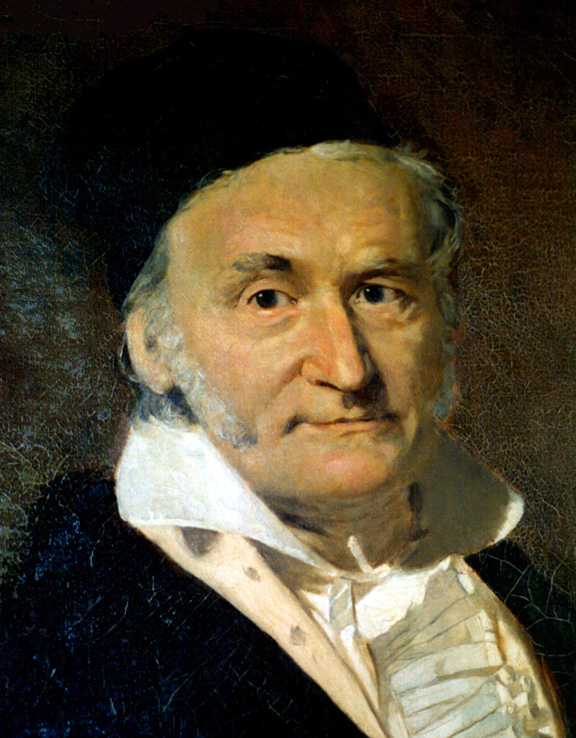
\includegraphics[height=5cm, width=3.5cm]{gauss}
	\end{tabular}
	& \begin{tabular}{l}
		\parbox{0.5\linewidth}{%  change the parbox width as appropiate
			``The problem of distinguishing prime numbers from composite numbers \ldots is known to be one of the most important and useful in arithmetic. \ldots Further, the dignity of the science itself seems to require that every possible means be explored for the solution of a problem so elegant and so celebrated." --- \textit{Disquisitiones Arithmeticae (1801): Article 329} 
		}
	\end{tabular}  \\
\end{tabular}	
\end{frame}

\tikzset{
 	invisible/.style={opacity=0},
 	visible on/.style={alt={#1{}{invisible}}},
 	alt/.code args={<#1>#2#3}{%
 		\alt<#1>{\pgfkeysalso{#2}}{\pgfkeysalso{#3}} % \pgfkeysalso doesn't change the path
 	},
}

\begin{frame}
	\begin{center}

		\resizebox{!}{0.9\textheight}{%
			
	
			\begin{tikzpicture}
			\path[mindmap,concept color=black,text=white]
			node[concept] {Background for Miller-Rabin Test}
			[clockwise from=0]
			child[concept color=blue] { node[concept](congruence) {Congruence Classes} }			
			child[concept color=green!50!black] {
				node[concept] {Divisibility}
				[clockwise from=0]
				child[visible on=<2->] { node[concept](gcd) {GCD} }
				child[visible on=<3->] { node[concept](combos) {Linear Combinations} }
			}
			child[concept color=orange] { node[concept] {Algebraic Structures}
				[clockwise from=-90]
				child[visible on=<5->] { node[concept] {Monoid} 
					child[grow=-45] { node[concept] {Set} }
					child[grow=-90] { node[concept] {Associative Binary Operation} }
					child[grow=-135, visible on=<6->] { node[concept] {Identity Element} }
					}
				child[visible on=<7->] { node[concept] {Abelian Group} 
					child[grow=-110] { node[concept] {Monoid} }
					child[grow=-155] { node[concept] {Inverses} }
					child[grow=-200, visible on=<8->]{ node[concept] {Commu-tative Operation} }
					}
				child[visible on=<9->] { node[concept] {Ring}
					[clockwise from=-180]
					child[grow=190] { node[concept] {Abelian Group Under Addition} }
					child[grow=140] { node[concept] {Monoid Under Multiplication} }
					child[grow=90, visible on=<10->] { node[concept] {Disribution} }
					}				
			};
			\draw [concept connection, visible on=<4->] (gcd) edge (combos);				
			\end{tikzpicture}
		}
	\end{center}

\end{frame}

\section{Structure of $\Z_n$}
\begin{frame}
	\frametitle{Congruence Example}

	\begin{definition}[Congruent]\label{definition:congruent}
		Let $a,b,n \in \Z$ with $n > 0$. We say that $a$ is congruent to $b$ modulo $n$ if $n \mid (a - b)$, denoted $a \equiv b \pmod n$. \cite{pommersheim}
	\end{definition}\pause
	
	\begin{example}\label{example:congruent}
		Is 34 congruent to 4 modulo 10?\pause
		
		Subtracting 4 from 34, we have $34 - 4 = 30$.
		
		Does $10$ divide this difference?\pause 
		
		Yes, since $30 = 3 \cdot 10$.
		
		Thus, $34 \equiv 4 \pmod{10}$.
	\end{example}
\end{frame}	

\begin{frame}
	\frametitle{The Set of All Congruence Classes}
	\begin{definition}[Congruence Class]\label{definition:congruence_class}
		%		Let $n \in \N$, and let $b \in \Z$. Then the \textbf{congruence class} of $b$ modulo $n$ is the set of all integers congruent to $b$ modulo $n$: $$ \bar{b} := \{ x \in \Z : x \equiv b \pmod n \}. $$ The congruence class of $b$ modulo $n$ may also be defined as $$ \bar{b} := \{ b + kn : k \in \Z \}. $$
		Let $a,n \in \Z$ with $n > 0$. We define the congruence class of $a$ modulo $n$ as the set of all integers congruent to $a$ modulo $n$; that is, $$\bar{a} := \{ x \in \Z : x \equiv a \pmod n \}.$$% $$ \bar{a} := \{ a + kn : k \in \Z \}.$$
	\end{definition}\pause
	
	\begin{definition}[$\Z_n$]\label{Definition: Zn}
		Let $n > 0$ be any integer. We define $\Z_n$ to be the set of all congruence classes modulo $n$, i.e. $$ \Z_n := \{ \bar{0}, \bar{1}, \bar{2}, \ldots, \overline{n - 1} \}.$$
	\end{definition}

\end{frame}

\begin{frame}
	\frametitle{$\Z_n$ Is an Abelian Group under Addition}
	
	\begin{center}
		\resizebox{!}{0.85\textheight}{%		
			\begin{tikzpicture}
			\path[mindmap,concept color=black,text=white]
			node[concept] {Background for Miller-Rabin Test}
			[clockwise from=0]
			child[concept color=gray!50] {
				node[concept] {Divisibility}
				[clockwise from=0]
				child { node[concept] {GCD} }
				child { node[concept] {Linear Combinations} }
			}
			child[concept color=blue] { node[concept](congruence) {Congruence Classes} }
			child[concept color=orange] { node[concept] {Algebraic Structures}
				[clockwise from=-90]
				child[concept color=gray!50] { node[concept] {Monoid} 
					child[grow=-45] { node[concept] {Set} }
					child[grow=-90] { node[concept] {Associative Binary Operation} }
					child[grow=-135] { node[concept] {Identity Element} }
				}
				child { node[concept](group) {Abelian Group} 
					child[grow=-110] { node[concept] {Monoid} }
					child[grow=-155] { node[concept] {Inverses} }
					child[grow=-200]{ node[concept] {Commu-tative Operation} }
				}
				child[concept color=gray!50] { node[concept] {Ring}
					[clockwise from=-180]
					child[grow=190] { node[concept] {Abelian Group Under Addition} }
					child[grow=140] { node[concept] {Monoid Under Multiplication} }
					child[grow=90] { node[concept] {Disribution} }
				}				
			};
			\draw [concept connection] (congruence) edge (group);						
			\end{tikzpicture}
		}
	\end{center}
	
\end{frame}


%\begin{frame}
%	\frametitle{$\Z_n$ Is a Monoid under Multiplication}
%	\begin{center}
%		\resizebox{!}{0.85\textheight}{%		
%			\begin{tikzpicture}
%			\path[mindmap,concept color=black,text=white]
%			node[concept] {Background for Miller-Rabin Test}
%			[clockwise from=0]
%			child[concept color=gray!50] {
%				node[concept] {Divisibility}
%				[clockwise from=0]
%				child { node[concept] {GCD} }
%				child { node[concept] {Linear Combinations} }
%			}
%			child[concept color=blue] { node[concept](congruence) {Congruence Classes} }
%			child[concept color=orange] { node[concept] {Algebraic Structures}
%				[clockwise from=-90]
%				child { node[concept] (monoid) {Monoid} 
%					child[grow=-45] { node[concept] {Set} }
%					child[grow=-90] { node[concept] {Associative Binary Operation} }
%					child[grow=-135] { node[concept] {Identity Element} }
%				}
%				child[concept color=gray!50] { node[concept] {Abelian Group} 
%					child[grow=-110] { node[concept] {Monoid} }
%					child[grow=-155] { node[concept] {Inverses} }
%					child[grow=-200]{ node[concept] {Commu-tative Operation} }
%				}
%				child[concept color=gray!50] { node[concept] {Ring}
%					[clockwise from=-180]
%					child[grow=190] { node[concept] {Abelian Group Under Addition} }
%					child[grow=140] { node[concept] {Monoid Under Multiplication} }
%					child[grow=90] { node[concept] {Disribution} }
%				}				
%			};
%
%			\draw [concept connection] (congruence) edge (monoid);
%
%			\end{tikzpicture}
%		}
%	\end{center}
%\end{frame}

\begin{frame}
	\frametitle{$\Z_n$ Is a Monoid under Multiplication}
	
	\begin{itemize}
		\item $ \bar{a} \cdot \bar{b} := \overline{a \cdot b}.$\pause
		\item By the associativity of integer multiplication, we have 
		\begin{align*}
		(\bar{a} \cdot \bar{b}) \cdot \bar{c} 
		&= \overline{a \cdot b} \cdot \bar{c} \\
		&= \overline{(a \cdot b) \cdot c} \\
		&= \overline{a \cdot (b \cdot c)} \\
		&= \bar{a} \cdot \overline{b \cdot c} \\
		&= \bar{a} \cdot (\bar{b} \cdot \bar{c}).
		\end{align*}\pause
		\item Since $(n+1) = 1 + kn$ for $k=1 \in \Z$, we know $(n+1) \equiv 1 \pmod n$, which is en element in $\bar{1} \in \Z_n$.
	\end{itemize}

\end{frame}

%
%\begin{frame}
%	\frametitle{$\Z_n$ Is an Abelian Group under Addition}
%	\begin{itemize}
%		\item $ \bar{a} + \bar{b} := \overline{a + b}$\pause
%		\item By the associativity of addition on the integers, we have 
%		\begin{align*}
%		(\bar{a} + \bar{b}) + \bar{c} = \overline{a + b}  + \bar{c} 
%		&= \overline{(a + b) + c} = \overline{a + (b + c)} \\
%		&= \bar{a} + \overline{b + c} = \bar{a} + (\bar{b} + \bar{c})
%		\end{align*}\pause
%		\item Inverses
%		\begin{align*}
%		\bar{a} + \overline{n-a} 
%		= \overline{a + n - a}
%		&= \bar{n} \\
%		&= \overline{n + (-a) + a}
%		= \overline{n-a} + \bar{a}
%		\end{align*}\pause
%		\item $\bar{a}+\bar{b} = \overline{a + b} = \overline{b + a} = \bar{b} + \bar{a}$
%	\end{itemize}
%\end{frame}

\begin{frame}
	\frametitle{Multiplication Distributes over Addition}

	\begin{itemize}
		\item Left Distribution
		\begin{align*}
		\bar{a} \cdot (\bar{b}+\bar{c}) 
		= \bar{a} \cdot \overline{b+c}
		= \overline{a (b+c)}
		&= \overline{a \cdot b+ac} \\
		&= \overline{a \cdot b} + \overline{a \cdot c} \\
		&= \bar{a} \cdot \bar{b} + \bar{a} \cdot \bar{c}
		\end{align*}\pause
		
		\item Right Distribution
		\begin{align*}
		(\bar{a}+\bar{b}) \cdot \bar{c} 
		= \overline{a + b} \cdot \bar{c} 
		= \overline{(a + b)c} 
		&= \overline{a \cdot c + b \cdot c} \\
		&= \overline{a \cdot c} + \overline{b \cdot c} \\
		&= \bar{a} \cdot \bar{c} + \bar{b} \cdot \bar{c}
		\end{align*}	
	\end{itemize}
\end{frame}

\begin{frame}
	\frametitle{$\Z_n$ Is a Ring}
	\begin{center}
		\resizebox{!}{0.85\textheight}{%		
			\begin{tikzpicture}
			\path[mindmap,concept color=black,text=white]
			node[concept] {Background for Miller-Rabin Test}
			[clockwise from=0]
			child[concept color=gray!50] {
				node[concept] {Divisibility}
				[clockwise from=0]
				child { node[concept] {GCD} }
				child { node[concept] {Linear Combinations} }
			}
			child[concept color=blue] { node[concept](congruence) {Congruence Classes} }
			child[concept color=orange] { node[concept] {Algebraic Structures}
				[clockwise from=-90]
				child[concept color=gray!50] { node[concept] {Monoid} 
					child[grow=-45] { node[concept] {Set} }
					child[grow=-90] { node[concept] {Associative Binary Operation} }
					child[grow=-135] { node[concept] {Identity Element} }
				}
				child[concept color=gray!50] { node[concept] {Abelian Group} 
					child[grow=-110] { node[concept] {Monoid} }
					child[grow=-155] { node[concept] {Inverses} }
					child[grow=-200]{ node[concept] {Commu-tative Operation} }
				}
				child { node[concept](ring) {Ring}
					[clockwise from=-180]
					child[grow=190] { node[concept] {Abelian Group Under Addition} }
					child[grow=140] { node[concept] {Monoid Under Multiplication} }
					child[grow=90] { node[concept] {Disribution} }
				}				
			};
			\draw [concept connection] (congruence) edge (ring);						
			\end{tikzpicture}
		}
	\end{center}	
\end{frame}

\begin{frame}
	\frametitle{$\Z_p$: When $n$ Is Prime}	
	
	\begin{table}[h!]
		\centering
		\begin{minipage}{0.48\textwidth}
			\centering
			\caption{Multiplication in $\Z_7$}
			\label{Multiplication in Z_7}
			\begin{tabular}{|c|c|c|c|c|c|c|c|}
				\hline
				$\cdot$		& $\bar{0}$ & $\bar{1}$ & $\bar{2}$ & $\bar{3}$ & $\bar{4}$ & $\bar{5}$ & $\bar{6}$ \\ \hline
				$\bar{0}$	& $\bar{0}$ & $\bar{0}$ & $\bar{0}$ & $\bar{0}$ & $\bar{0}$ & $\bar{0}$ & $\bar{0}$ \\ \hline
				$\bar{1}$	& $\bar{0}$ & $\bar{1}$\cellcolor{yellow} & $\bar{2}$ & $\bar{3}$ & $\bar{4}$ & $\bar{5}$ & $\bar{6}$ \\ \hline
				
				$\bar{2}$	& $\bar{0}$ & $\bar{2}$ & $\bar{4}$ & $\bar{6}$ & $\bar{1}$\cellcolor{yellow} & $\bar{3}$ & $\bar{5}$ \\ \hline
				
				$\bar{3}$	& $\bar{0}$ & $\bar{3}$ & $\bar{6}$ & $\bar{2}$ & $\bar{5}$ & $\bar{1}$\cellcolor{yellow} & $\bar{4}$ \\ \hline
				
				$\bar{4}$	& $\bar{0}$ & $\bar{4}$ & $\bar{1}$\cellcolor{yellow} & $\bar{5}$ & $\bar{2}$ & $\bar{6}$ & $\bar{3}$ \\ \hline
				
				$\bar{5}$	& $\bar{0}$ & $\bar{5}$ & $\bar{3}$ & $\bar{1}$\cellcolor{yellow} & $\bar{6}$ & $\bar{4}$ & $\bar{2}$ \\ \hline
				
				$\bar{6}$	& $\bar{0}$ & $\bar{6}$ & $\bar{5}$ & $\bar{4}$ & $\bar{3}$ & $\bar{2}$ & $\bar{1}$\cellcolor{yellow} \\ \hline
			\end{tabular}
		\end{minipage}
		\hfill
		\begin{minipage}{0.48\textwidth}
			\centering
			\caption{Multiplication in $\Z_8$}
			\label{Multiplication in Z_8}
			\begin{tabular}{|c|c|c|c|c|c|c|c|c|}
				\hline
				$\cdot$		& $\bar{0}$ & $\bar{1}$ & $\bar{2}$ & $\bar{3}$ & $\bar{4}$ & $\bar{5}$ & $\bar{6}$ & $\bar{7}$ \\ \hline
				
				$\bar{0}$	& $\bar{0}$ & $\bar{0}$ & $\bar{0}$ & $\bar{0}$ & $\bar{0}$ & $\bar{0}$ & $\bar{0}$ & $\bar{0}$ \\ \hline
				
				$\bar{1}$	& $\bar{0}$ & $\bar{1}$\cellcolor{yellow} & $\bar{2}$ & $\bar{3}$ & $\bar{4}$ & $\bar{5}$ & $\bar{6}$ & $\bar{7}$ \\ \hline
				
				$\bar{2}$	& $\bar{0}$ & $\bar{2}$ & $\bar{4}$ & $\bar{6}$ & $\bar{0}$ & $\bar{2}$ & $\bar{4}$ & $\bar{6}$ \\ \hline
				
				$\bar{3}$	& $\bar{0}$ & $\bar{3}$ & $\bar{6}$ & $\bar{1}$\cellcolor{yellow} & $\bar{4}$ & $\bar{7}$ & $\bar{2}$ & $\bar{5}$ \\ \hline
				
				$\bar{4}$	& $\bar{0}$ & $\bar{4}$ & $\bar{0}$ & $\bar{4}$ & $\bar{0}$ & $\bar{4}$ & $\bar{0}$ & $\bar{4}$ \\ \hline
				
				$\bar{5}$	& $\bar{0}$ & $\bar{5}$ & $\bar{2}$ & $\bar{7}$ & $\bar{4}$ & $\bar{1}$\cellcolor{yellow} & $\bar{6}$ & $\bar{3}$ \\ \hline
				
				$\bar{6}$	& $\bar{0}$ & $\bar{6}$ & $\bar{4}$ & $\bar{2}$ & $\bar{0}$ & $\bar{6}$ & $\bar{4}$ & $\bar{2}$ \\ \hline
				
				$\bar{7}$	& $\bar{0}$ & $\bar{7}$ & $\bar{6}$ & $\bar{5}$ & $\bar{4}$ & $\bar{3}$ & $\bar{2}$ & $\bar{1}$\cellcolor{yellow} \\ \hline
			\end{tabular}
		\end{minipage}
	\end{table}	
\end{frame}


\begin{frame}
	\frametitle{Multiplicative Inverses}
	\begin{center}
		\resizebox{!}{0.85\textheight}{%		
			\begin{tikzpicture}
			\path[mindmap,concept color=black,text=white]
			node[concept] {Background for Miller-Rabin Test}
			[clockwise from=0]
			child[concept color=green!50!black] {
				node[concept] {Divisibility}
				[clockwise from=0]
				child { node[concept](gcd) {GCD} }
				child { node[concept](combos) {Linear Combinations} }
			}
			child[concept color=gray!50] { node[concept](congruence) {Congruence Classes} }
			child[concept color=gray!50] { node[concept] {Algebraic Structures}
				[clockwise from=-90]
				child[concept color=gray!50] { node[concept] {Monoid} 
					child[grow=-45] { node[concept] {Set} }
					child[grow=-90] { node[concept] {Associative Binary Operation} }
					child[grow=-135] { node[concept] {Identity Element} }
				}
				child { node[concept] {Abelian Group} 
					child[grow=-110] { node[concept] {Monoid} }
					child[grow=-155] { node[concept] {Inverses} }
					child[grow=-200]{ node[concept] {Commu-tative Operation} }
				}
				child { node[concept](ring) {Ring}
					[clockwise from=-180]
					child[grow=190] { node[concept] {Abelian Group Under Addition} }
					child[grow=140] { node[concept] {Monoid Under Multiplication} }
					child[grow=90] { node[concept] {Disribution} }
				}				
			};
			\draw [concept connection] (gcd) edge (combos);						
			\end{tikzpicture}
		}
	\end{center}	
\end{frame}

\begin{frame}
	\frametitle{Multiplicative Inverses}
	
	\begin{itemize}
		\item $\gcd(a,p)=1$
		\item $ax + py = 1$
		\item $ax = 1 + (-y)p$ or $ax \equiv 1 \pmod p$ 
		\item Thus, $\overline{a \cdot x} = \bar{a} \cdot \bar{x} = \bar{1}$.
	\end{itemize}
		
\end{frame}


\begin{frame}
	\frametitle{Zero Product Property}	
	
	\begin{itemize}
		\item If both $\bar{a} = \bar{0}$ and $\bar{b} = \bar{0}$, then $$\bar{a} \cdot \bar{b} = \bar{0} \cdot \bar{0} = \overline{0 \cdot 0} = \bar{0}.$$\pause
		\item If $\bar{a} \neq \bar{0}$, then 
		\begin{align*}
		\bar{a} \cdot \bar{b} &= \bar{0} \\
		\bar{a}^{-1} \cdot \bar{a} \cdot \bar{b} &= \bar{a}^{-1} \cdot \bar{0} \\
		\bar{b} &= \bar{0}.
		\end{align*}\pause
		
		\item 
		If $\bar{b} \neq \bar{0}$, then 
		\begin{align*}
		\bar{a} \cdot \bar{b} &= \bar{0} \\
		\bar{a} \cdot \bar{b} \cdot \bar{b}^{-1} &= \bar{0} \cdot \bar{b}^{-1} \\
		\bar{a} &= \bar{0}. \\
		\end{align*}
	\end{itemize}
	
\end{frame}

\begin{frame}
	\frametitle{A Pattern Perceptable}	
	\begin{table}[h!]
		\centering
		\begin{minipage}{0.48\textwidth}
			\centering
			\caption{Exponents in $\Z_5$}
			\begin{tabular}{|l|l|l|l|l|l|}
				\hline
				$\bar{a}$ 		& $\bar{0}$ & $\bar{1}$ & $\bar{2}$ & $\bar{3}$ & $\bar{4}$ \\ \hline
				$\bar{a}^2$ 	& $\bar{0}$ & $\bar{1}$ & $\bar{4}$ & $\bar{4}$ & $\bar{1}$ \\ \hline
				$\bar{a}^3$ 	& $\bar{0}$ & $\bar{1}$ & $\bar{3}$ & $\bar{2}$ & $\bar{4}$ \\ \hline	
				$\bar{a}^4$ 	& $\bar{0}$ & $\bar{1}$\cellcolor{yellow} & $\bar{1}$\cellcolor{yellow} & $\bar{1}$\cellcolor{yellow} & $\bar{1}$\cellcolor{yellow} \\ \hline
			\end{tabular}

		\end{minipage}
		\hfill
		\begin{minipage}{0.48\textwidth}
			\centering
			\caption{Exponents in $\Z_6$}
			\begin{tabular}{|l|l|l|l|l|l|l|}
				\hline
				$\bar{a}$ 		& $\bar{0}$ & $\bar{1}$ & $\bar{2}$ & $\bar{3}$ & $\bar{4}$ & $\bar{5}$ \\ \hline
				$\bar{a}^2$ 	& $\bar{0}$ & $\bar{1}$ & $\bar{4}$ & $\bar{3}$ & $\bar{4}$ & $\bar{1}$ \\ \hline
				$\bar{a}^3$ 	& $\bar{0}$ & $\bar{1}$ & $\bar{2}$ & $\bar{3}$ & $\bar{4}$ & $\bar{5}$ \\ \hline	
				$\bar{a}^4$ 	& $\bar{0}$ & $\bar{1}$ & $\bar{4}$ & $\bar{3}$ & $\bar{4}$ & $\bar{1}$ \\ \hline
				$\bar{a}^5$ 	& $\bar{0}$ & $\bar{1}$\cellcolor{yellow} & $\bar{2}$ & $\bar{3}$ & $\bar{4}$ & $\bar{5}$ \\ \hline			
			\end{tabular}
		\end{minipage}
	\end{table}	
\end{frame}

%	\begin{table}[]
%		\centering
%		\caption{Exponents in $\Z_5$}
%		\begin{tabular}{|l|l|l|l|l|l|}
%			\hline
%			$\bar{a}$ 		& $\bar{0}$ & $\bar{1}$ & $\bar{2}$ & $\bar{3}$ & $\bar{4}$ \\ \hline
%			$\bar{a}^2$ 	& $\bar{0}$ & $\bar{1}$ & $\bar{4}$ & $\bar{4}$ & $\bar{1}$ \\ \hline
%			$\bar{a}^3$ 	& $\bar{0}$ & $\bar{1}$ & $\bar{3}$ & $\bar{2}$ & $\bar{4}$ \\ \hline	
%			$\bar{a}^4$ 	& $\bar{0}$ & $\bar{1}$\cellcolor{yellow} & $\bar{1}$\cellcolor{yellow} & $\bar{1}$\cellcolor{yellow} & $\bar{1}$\cellcolor{yellow} \\ \hline
%		\end{tabular}
%	\end{table}
%\end{frame}
%
%\begin{frame}
%	\frametitle{A Pattern Perceptable}
%	\begin{table}[]
%		\centering
%		\caption{Exponents in $\Z_6$}
%		\begin{tabular}{|l|l|l|l|l|l|l|}
%			\hline
%			$\bar{a}$ 		& $\bar{0}$ & $\bar{1}$ & $\bar{2}$ & $\bar{3}$ & $\bar{4}$ & $\bar{5}$ \\ \hline
%			$\bar{a}^2$ 	& $\bar{0}$ & $\bar{1}$ & $\bar{4}$ & $\bar{3}$ & $\bar{4}$ & $\bar{1}$ \\ \hline
%			$\bar{a}^3$ 	& $\bar{0}$ & $\bar{1}$ & $\bar{2}$ & $\bar{3}$ & $\bar{4}$ & $\bar{5}$ \\ \hline	
%			$\bar{a}^4$ 	& $\bar{0}$ & $\bar{1}$ & $\bar{4}$ & $\bar{3}$ & $\bar{4}$ & $\bar{1}$ \\ \hline
%			$\bar{a}^5$ 	& $\bar{0}$ & $\bar{1}$\cellcolor{yellow} & $\bar{2}$ & $\bar{3}$ & $\bar{4}$ & $\bar{5}$ \\ \hline			
%		\end{tabular}
%	\end{table}
%\end{frame}

\begin{frame}[allowframebreaks]
	\frametitle{Fermat's Little Theorem}
	
	\begin{theorem}[Fermat's Little Theorem]\label{theorem:fermats_little_theorem}
		Let $p$ be prime, and let $\bar{a} \in \Z_p$ with $\bar{a} \neq \bar{0}$. Then $$ \bar{a}^{p-1} = \bar{1}.$$
	\end{theorem}

	\begin{proofs}
		Let $p$ be prime, and let $\bar{a} \in \Z_p, \bar{a} \neq \bar{0}$.
		We know that $\Z_p$ contains a unique inverse for each of its elements.
		Furthermore, $\bar{1}^{-1} = \bar{1}$ and $\overline{p-1}^{-1} = \overline{p-1}$.
		Thus, $\bar{1} \cdot \bar{2} \cdot \bar{3} \cdots \overline{p-1} = \bar{1} \cdot \overline{p-1} = \overline{p-1}$.
		Then 
		\begin{align*}
		(\bar{a} \cdot \bar{1})(\bar{a} \cdot \bar{2}) \cdots (\bar{a} \cdot \overline{p-1})
		&= \underbrace{\bar{a} \cdot \bar{a} \cdots \bar{a}}_{p-1 \text{ times}} \cdot \bar{1} \cdot \bar{2} \cdots \bar{a} \cdots \bar{a}^{-1} \cdots \overline{p-1} \\
		&= \bar{a}^{p-1} \cdot \overline{p-1}.
		\end{align*}
		Moreover, since this multiplication is a bijection, we know that each product is equal to a unique element in $\Z_p$.
		Thus, $(\bar{a} \cdot \bar{1})(\bar{a} \cdot \bar{2}) \cdots (\bar{a} \cdot \overline{p-1}) = \bar{1} \cdot \bar{2} \cdots \overline{p-1}$, where the right-hand side is some permutation of the elements in $\Z_p$.
	\end{proofs}
	
	\begin{proofs}[\proofname\ (Cont.)]
		Hence,
		\begin{align*}
		\bar{a}^{p-1} \cdot \overline{p-1} 
		&= \bar{1} \cdot \bar{2} \cdots \overline{p-1} \\
		\bar{a}^{p-1} \cdot \overline{p-1}
		&= \overline{p-1} \\
		\bar{a}^{p-1}\cdot \overline{p-1} \cdot \overline{p-1}
		&= \overline{p-1}	\cdot \overline{p-1} \\
		\bar{a}^{p-1}\cdot \bar{1} 
		&= \bar{1}  \\
		\bar{a}^{p-1}
		&= \bar{1}.
		\end{align*}
		Therefore, if $p$ is prime, then $\bar{a}^{p-1} = \bar{1}$ for all $\bar{a} \in \Z_p, \bar{a} \neq \bar{0}$.
	\end{proofs}
		
\end{frame}

\begin{frame}
	\frametitle{Review}
%	\begin{itemize}
%		\item $\Z_n$ is a ring.\pause
%		\item Let $p$ be prime, then
%		\begin{itemize}
%			\item $\exists \bar{a}^{-1} \in \Z_p:$ $$\bar{a} \cdot \bar{a}^{-1} = \bar{a}^{-1} \cdot \bar{a} = \bar{1}$$ for all $\bar{a} \in \Z_p$, and\pause
%			\item $\bar{a}^{p-1} = \bar{1}$.
%		\end{itemize}
%	\end{itemize}
%	
	\begin{figure}[!htb]
		\minipage{0.32\textwidth}
		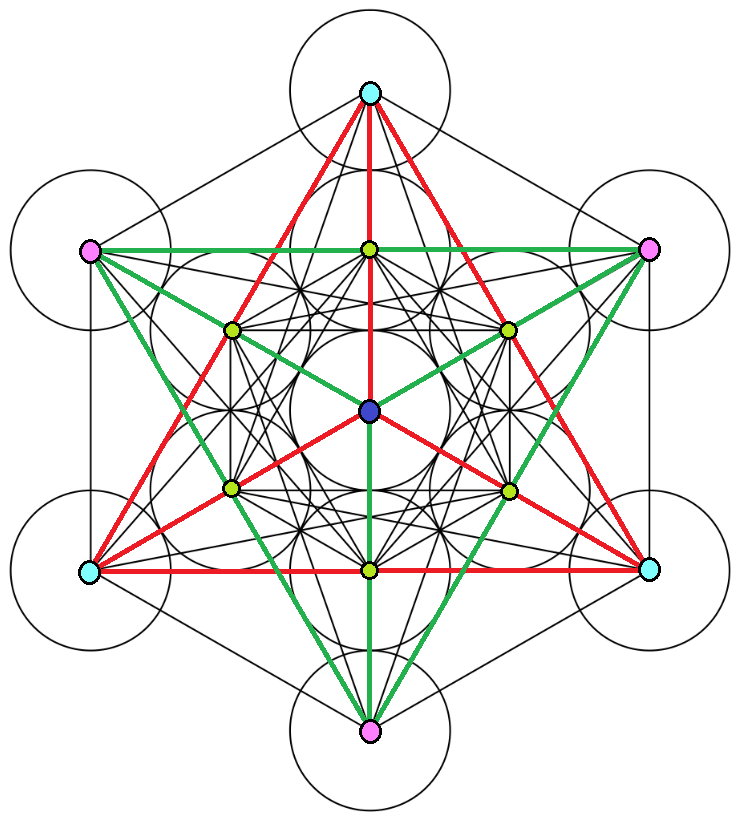
\includegraphics[width=\linewidth]{left_solid.png}
		\begin{center}
			$\Z_n$ is a ring.
		\end{center}
		%\caption{A really Awesome Image}\label{fig:awesome_image1}
		\endminipage\hfill\pause
		\noindent\fcolorbox{red}{gray}{%
		\minipage{0.32\textwidth}
		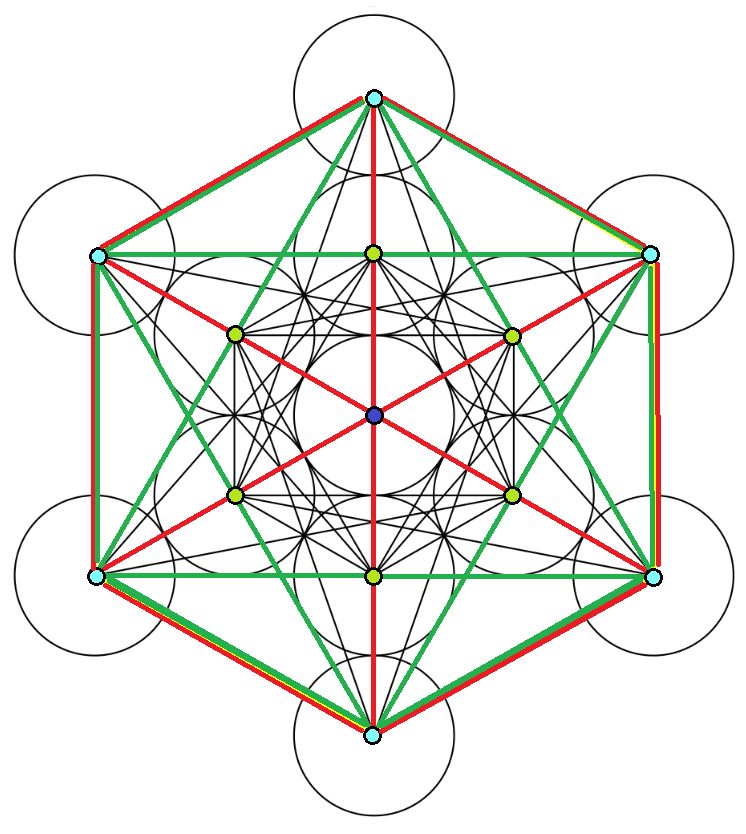
\includegraphics[width=\linewidth]{center_solid.png}
		\begin{center}
			\color{white}
			Let $p$ be prime. Then $\exists \bar{a}^{-1} \in \Z_p:$ $$\bar{a} \cdot \bar{a}^{-1} = \bar{a}^{-1} \cdot \bar{a} = \bar{1}$$ for all $\bar{a} \in \Z_p$
		\end{center}
		\endminipage}\hfill\pause
		\minipage{0.32\textwidth}%
		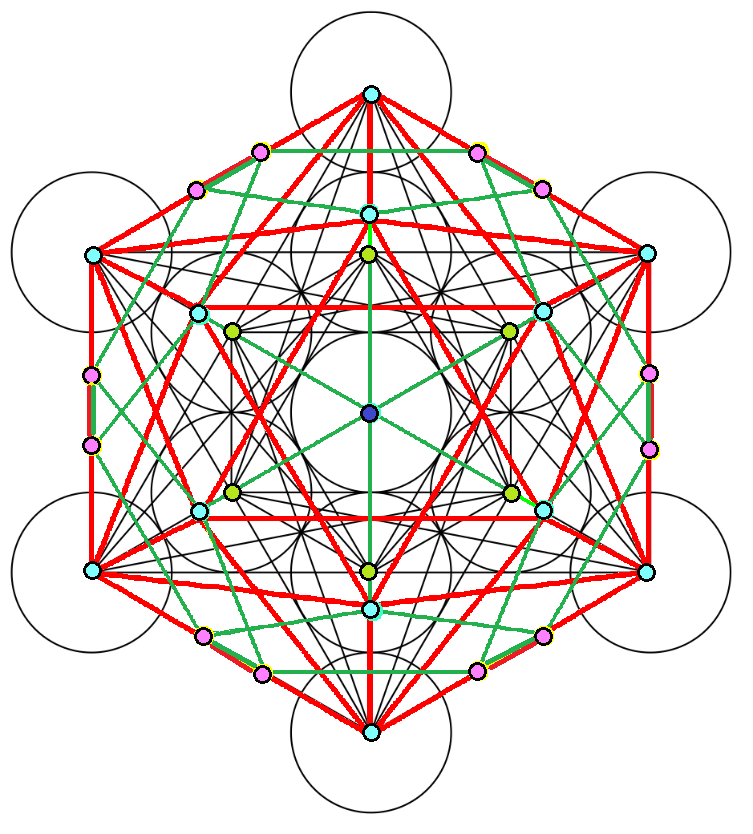
\includegraphics[width=\linewidth]{right_solid.png}
		\begin{center}
			Let $p$ be prime. Then $\bar{a}^{p-1} = \bar{1}$.
		\end{center}
		\endminipage
	\end{figure}	
\end{frame}

\section{Miller-Rabin Test}

\begin{frame}
	\frametitle{Example: Completing the Square in $\Z_{13}$}
	
	\begin{itemize}
		\item Choose $\bar{6} \in \Z_{13}$\pause
		\item Factor
		\begin{align*}
		\bar{6}^{13-1} &= \bar{1} \\
		\bar{6}^{12} - \bar{1} &= \bar{0} \\
		(\bar{6}^{6} + \bar{1}) \cdot (\bar{6}^{6} - \bar{1}) &= \bar{0} \\
		(\bar{6}^{6} + \bar{1}) \cdot (\bar{6}^{3} + \bar{1}) \cdot (\bar{6}^{3} - \bar{1}) &= \bar{0} 		
		\end{align*}\pause
		\item Zero product product property
		\begin{align*}
			(\bar{6}^{6} + \bar{1}) = \bar{0} &\iff \bar{6}^{6} = -\bar{1} \\
			(\bar{6}^{3} + \bar{1}) = \bar{0} &\iff \bar{6}^{3} = -\bar{1}\\
			(\bar{6}^{3} - \bar{1}) = \bar{0} &\iff \bar{6}^{3} = \bar{1}
		\end{align*}
	\end{itemize}
	
\end{frame}

\begin{frame}
	\frametitle{Miller-Rabin Test for Compositeness}

	\begin{algorithm}[Miller-Rabin Test for Compositeness]\label{algorithm:miller-rabin}
		Let $n>0$ be any odd integer. 
		Then there exists an integer $k > 0$ such that $2^k$ is that largest power of two that divides $n-1$.
		If there exists $\bar{a} \in \Z_n$ such that  
		$$\bar{a}^{\frac{n-1}{2^k}} \neq \bar{1}$$ and 
		$$\bar{a}^{\frac{n-1}{2^h}} \neq -\bar{1},$$ 
		for all $h \in \Z : 1 \leq h \leq k$, then $n$ is composite. 
		In this case, the integer $a$ is called a Miller-Rabin witness to the compositeness of $n$.
	\end{algorithm}
	
\end{frame}

\begin{frame}[allowframebreaks]
	\frametitle{Miller-Rabin Test Example}
	
	\begin{example}
		We would like to test the compositeness of 169. Since $2^3$ is the largest power of two that divides 168, we must find an $\bar{a}\in \Z_{169}$ such that $\bar{a}^{\frac{168}{2^3}} \neq \bar{1}$ and $\bar{a}^{\frac{168}{2^h}} \neq -\bar{1}$ for all $h$, $h=1,2,3$. So, we randomly choose $\overline{19} \in \Z_{169}$ and find that
		\begin{align*}
		\overline{19}^{\frac{168}{2^3}} = \overline{19}^{21} &= \overline{70} \\
		\overline{19}^{\frac{168}{2^3}} = \overline{19}^{21} &= \overline{70} \\
		\overline{19}^{\frac{168}{2^2}} = \overline{19}^{42} &= -\bar{1} \\
		\overline{19}^{\frac{168}{2^1}} = \overline{19}^{84} &= \bar{1}. \\
		\end{align*}
		\theorembreak
		Because $\overline{19}^{\frac{168}{2^2}} = -\bar{1}$, we cannot conclude that $169$ is composite. So we randomly select a different $\bar{a} \in \Z_{169}$, namely $\bar{a} = \overline{145}$, and this time discover that
		\begin{align*}
		\overline{145}^{\frac{168}{2^3}} = \overline{145}^{21} &= \overline{18} \\		
		\overline{145}^{\frac{168}{2^3}} = \overline{145}^{21} &= \overline{18} \\
		\overline{145}^{\frac{168}{2^2}} = \overline{145}^{42} &= \overline{155} \\
		\overline{145}^{\frac{168}{2^1}} = \overline{145}^{84} &= \overline{27}. \\
		\end{align*}
		Hence, $145$ is a Miller-Rabin witness to the compositeness of $169$ and we conclude that $169$ is not prime. 
	\end{example}
	
\end{frame}

\begin{frame}
	\frametitle{Effectiveness of the Miller-Rabin Test}
	\begin{itemize}
		\item At least $\frac{3}{4}$ of the integers $a$ in the range $1,2,\ldots,n-1$ are Miller-Rabin witnesses.
		\item If we run the test 100 times on a composite number, the probability that we will never find a witness is less than $\left( \frac{1}{4} \right)^{100} = 6.223 \times 10^{-61}$.
	\end{itemize}
	
	\begin{center}
		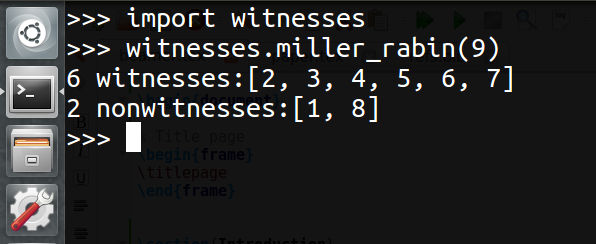
\includegraphics[width=0.7\textwidth]{miller_rabin_example}
	\end{center}
	
\end{frame}


\section{Support Vector Machine}

\begin{frame}
	\frametitle{Linear Classification with a Twist}
	\begin{itemize}
		\item Use non-linear function $K$ to map input vector to a higher dimensional feature space 
		
		\item Linear decision function with maximal margin between vectors of different classes
	
	\end{itemize}
	
	\begin{center}
		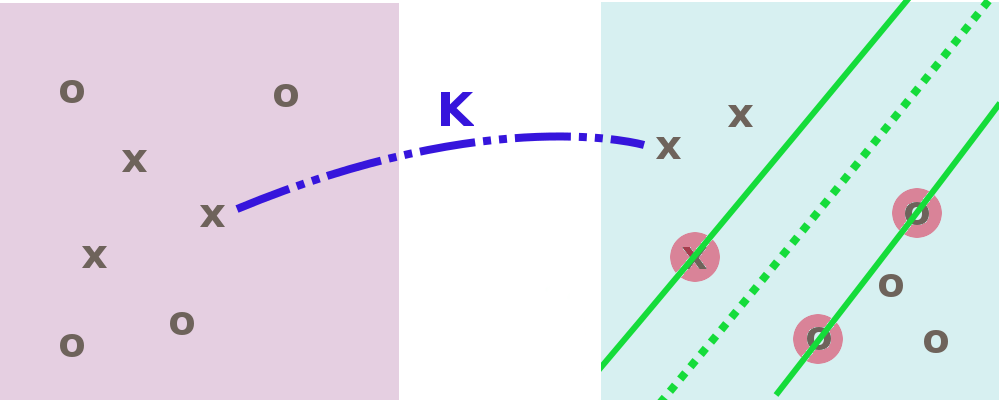
\includegraphics[width=\textwidth]{svm_graph}
	\end{center}
	
\end{frame}

\begin{frame}
	\frametitle{Training Methodology}
	
	\begin{itemize}
		\item Integer range: 2-1000 \pause
		\item 2,755,256 models using $$K(\vec{x}, \vec{x}^\prime) := \exp\left( -\gamma \lVert \vec{x} - \vec{x}^\prime \rVert^2 \right)$$ with $\gamma = \frac{1}{n}$, where $n$ is the length of the longest vector in the domain. \pause
		\item Base $b$ representations. For example, let $b = 6$. Then 
		\begin{align*}
			32 &\to (5,2) \\
			153 &\to (4,1,3) \\
			1000 &\to (4,3,4,4)
		\end{align*}\pause
		\item Class weight for primes
		\item Penalty parameter C
	\end{itemize}
\end{frame}


\begin{frame}
	\frametitle{Testing: Class Weight of Primes}
	\begin{center}
		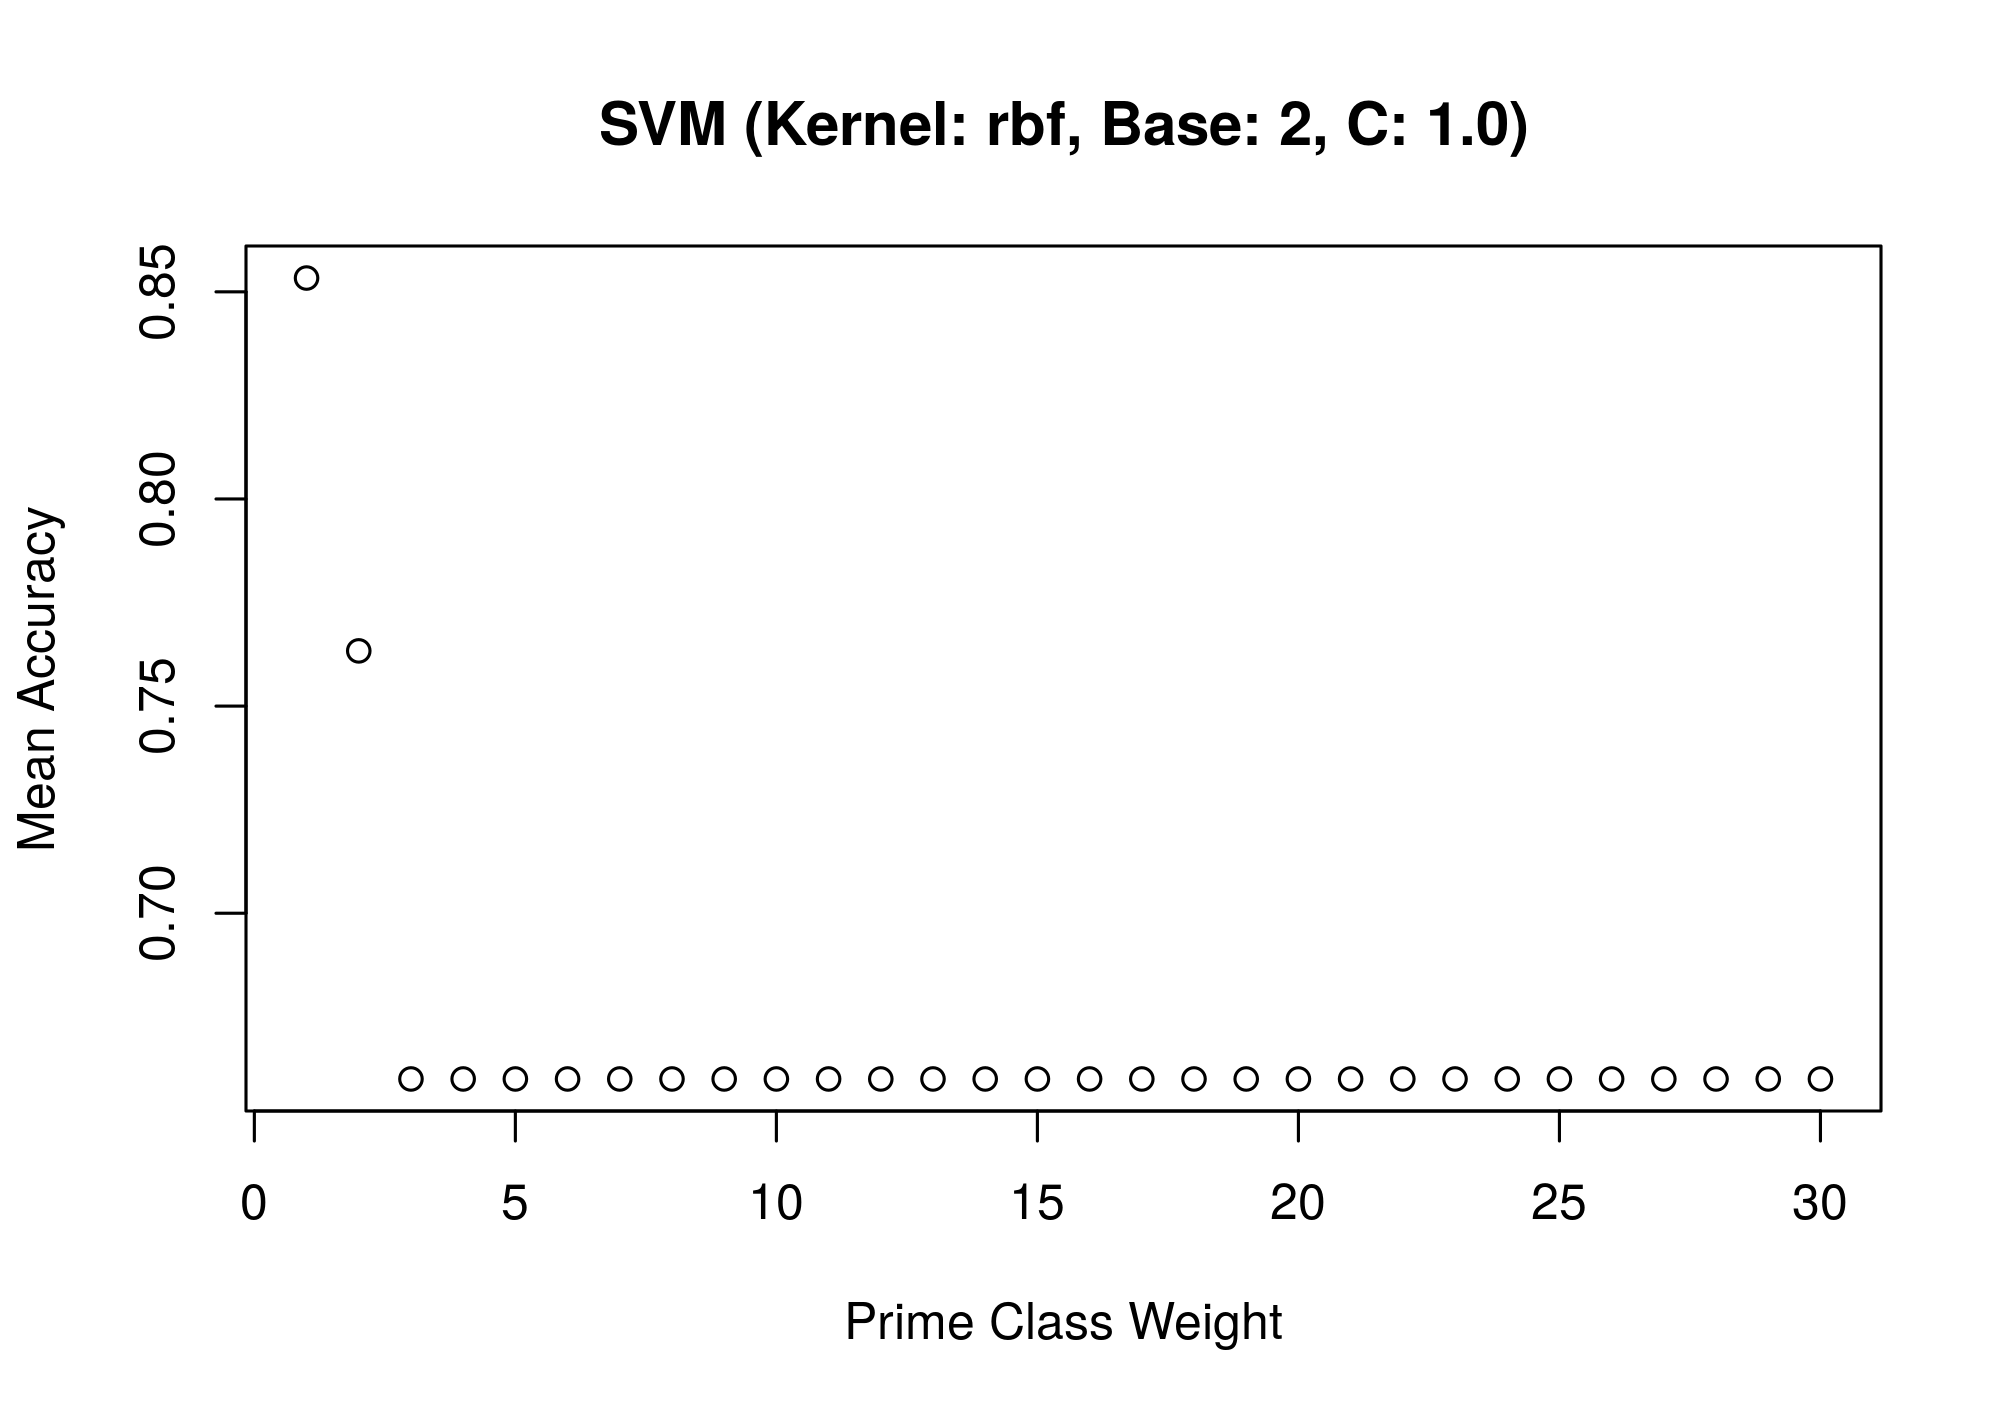
\includegraphics[width=\textwidth]{weight_demo}
	\end{center}
\end{frame}


\begin{frame}
	\frametitle{Testing: Penalty Parameter C}
	\begin{center}
		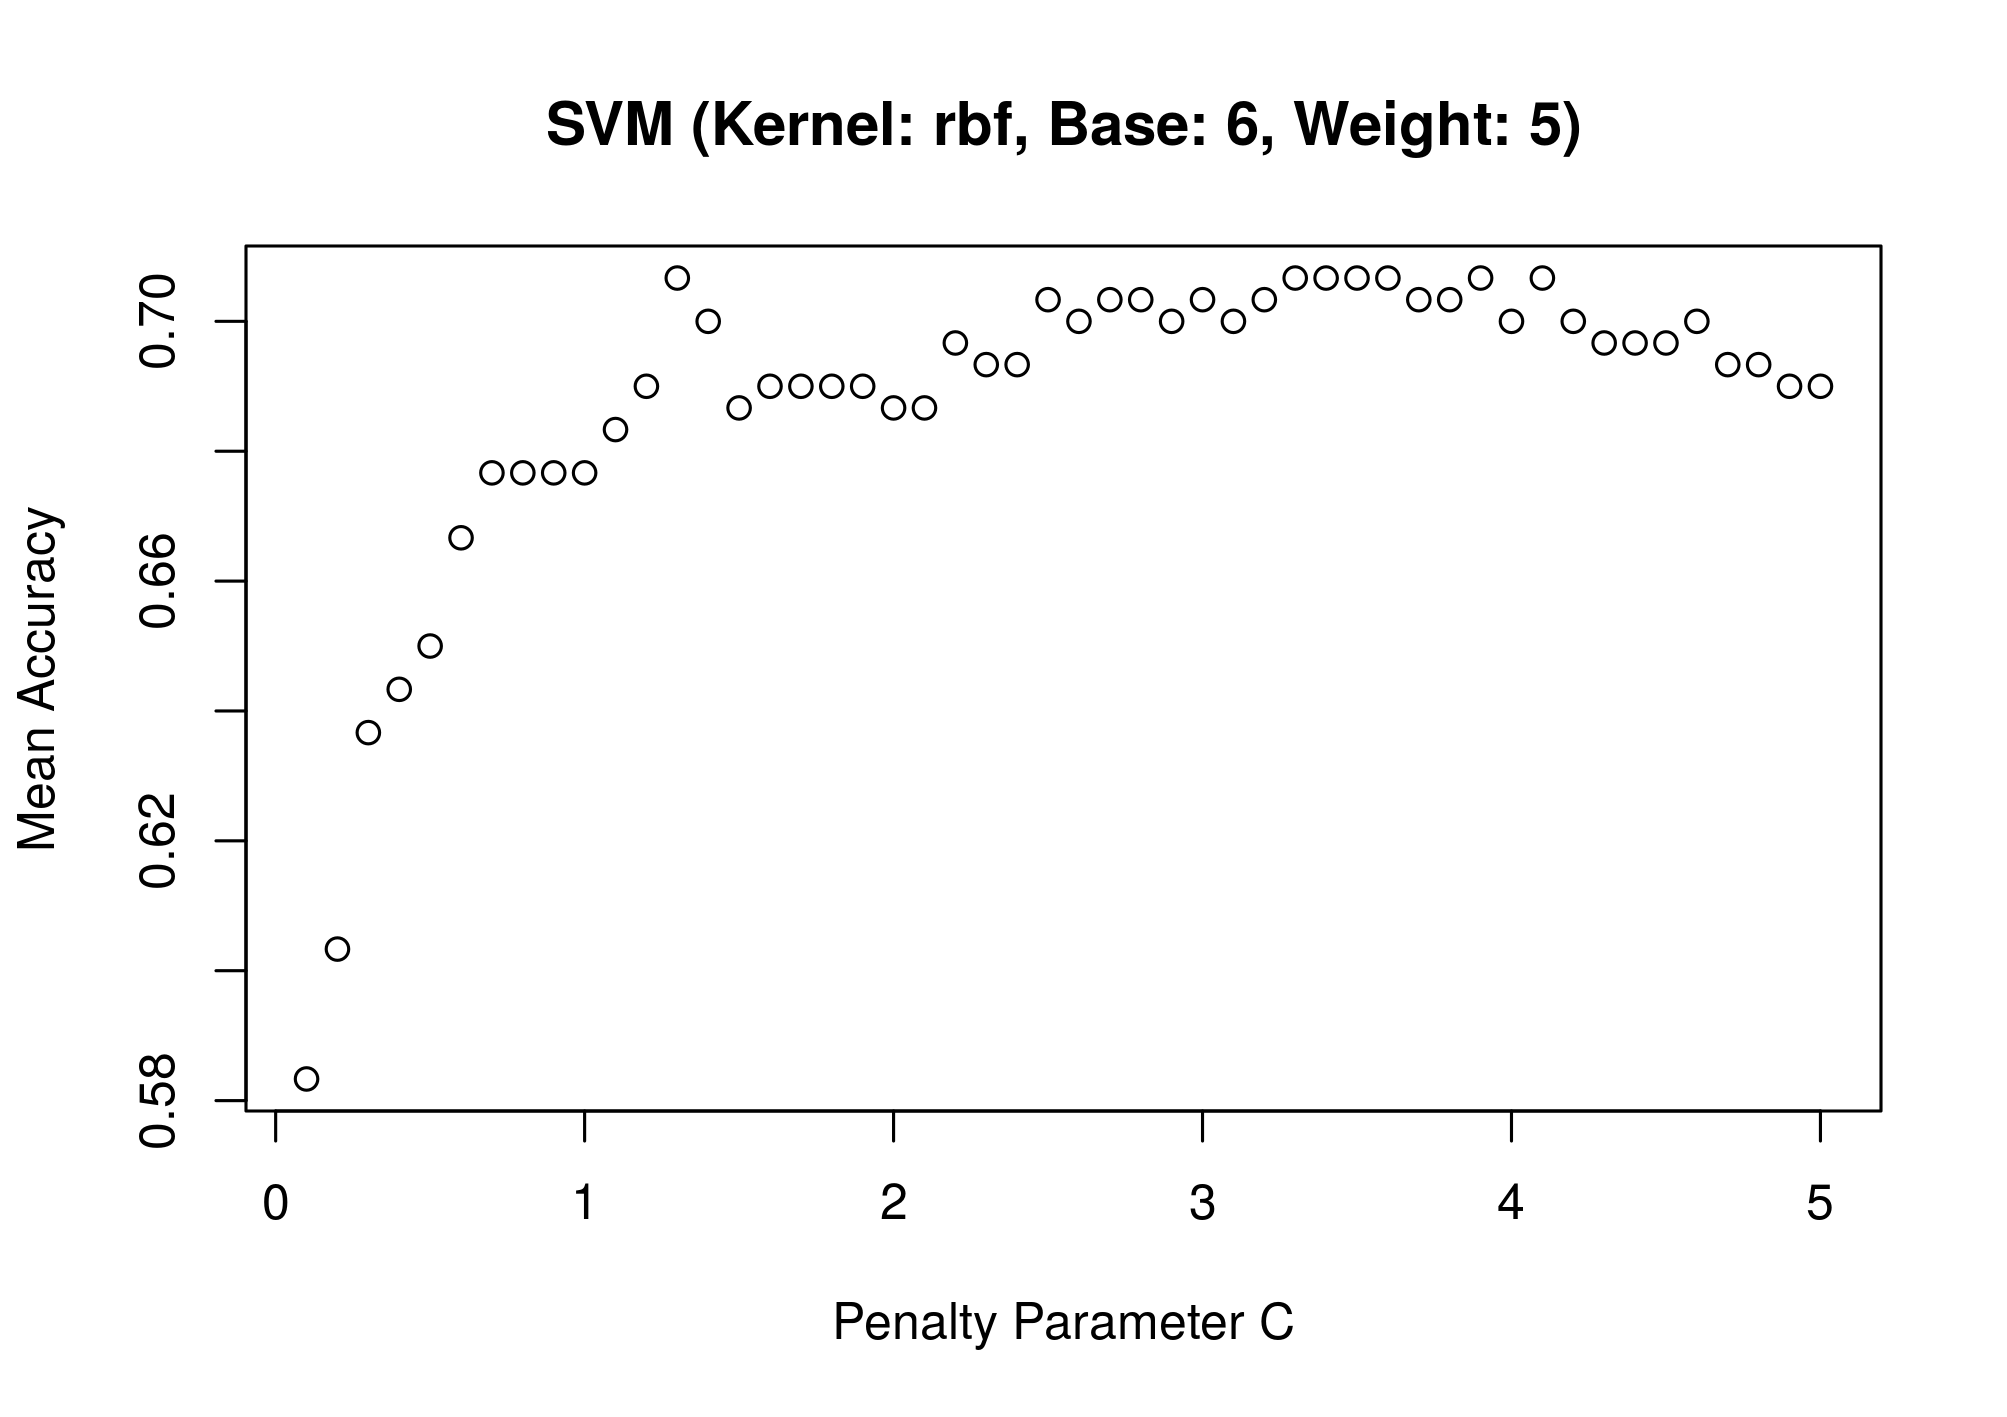
\includegraphics[width=\textwidth]{c_demo}
	\end{center}	
\end{frame}

\begin{frame}
	\frametitle{Testing: Base b Representations}
	\begin{center}
		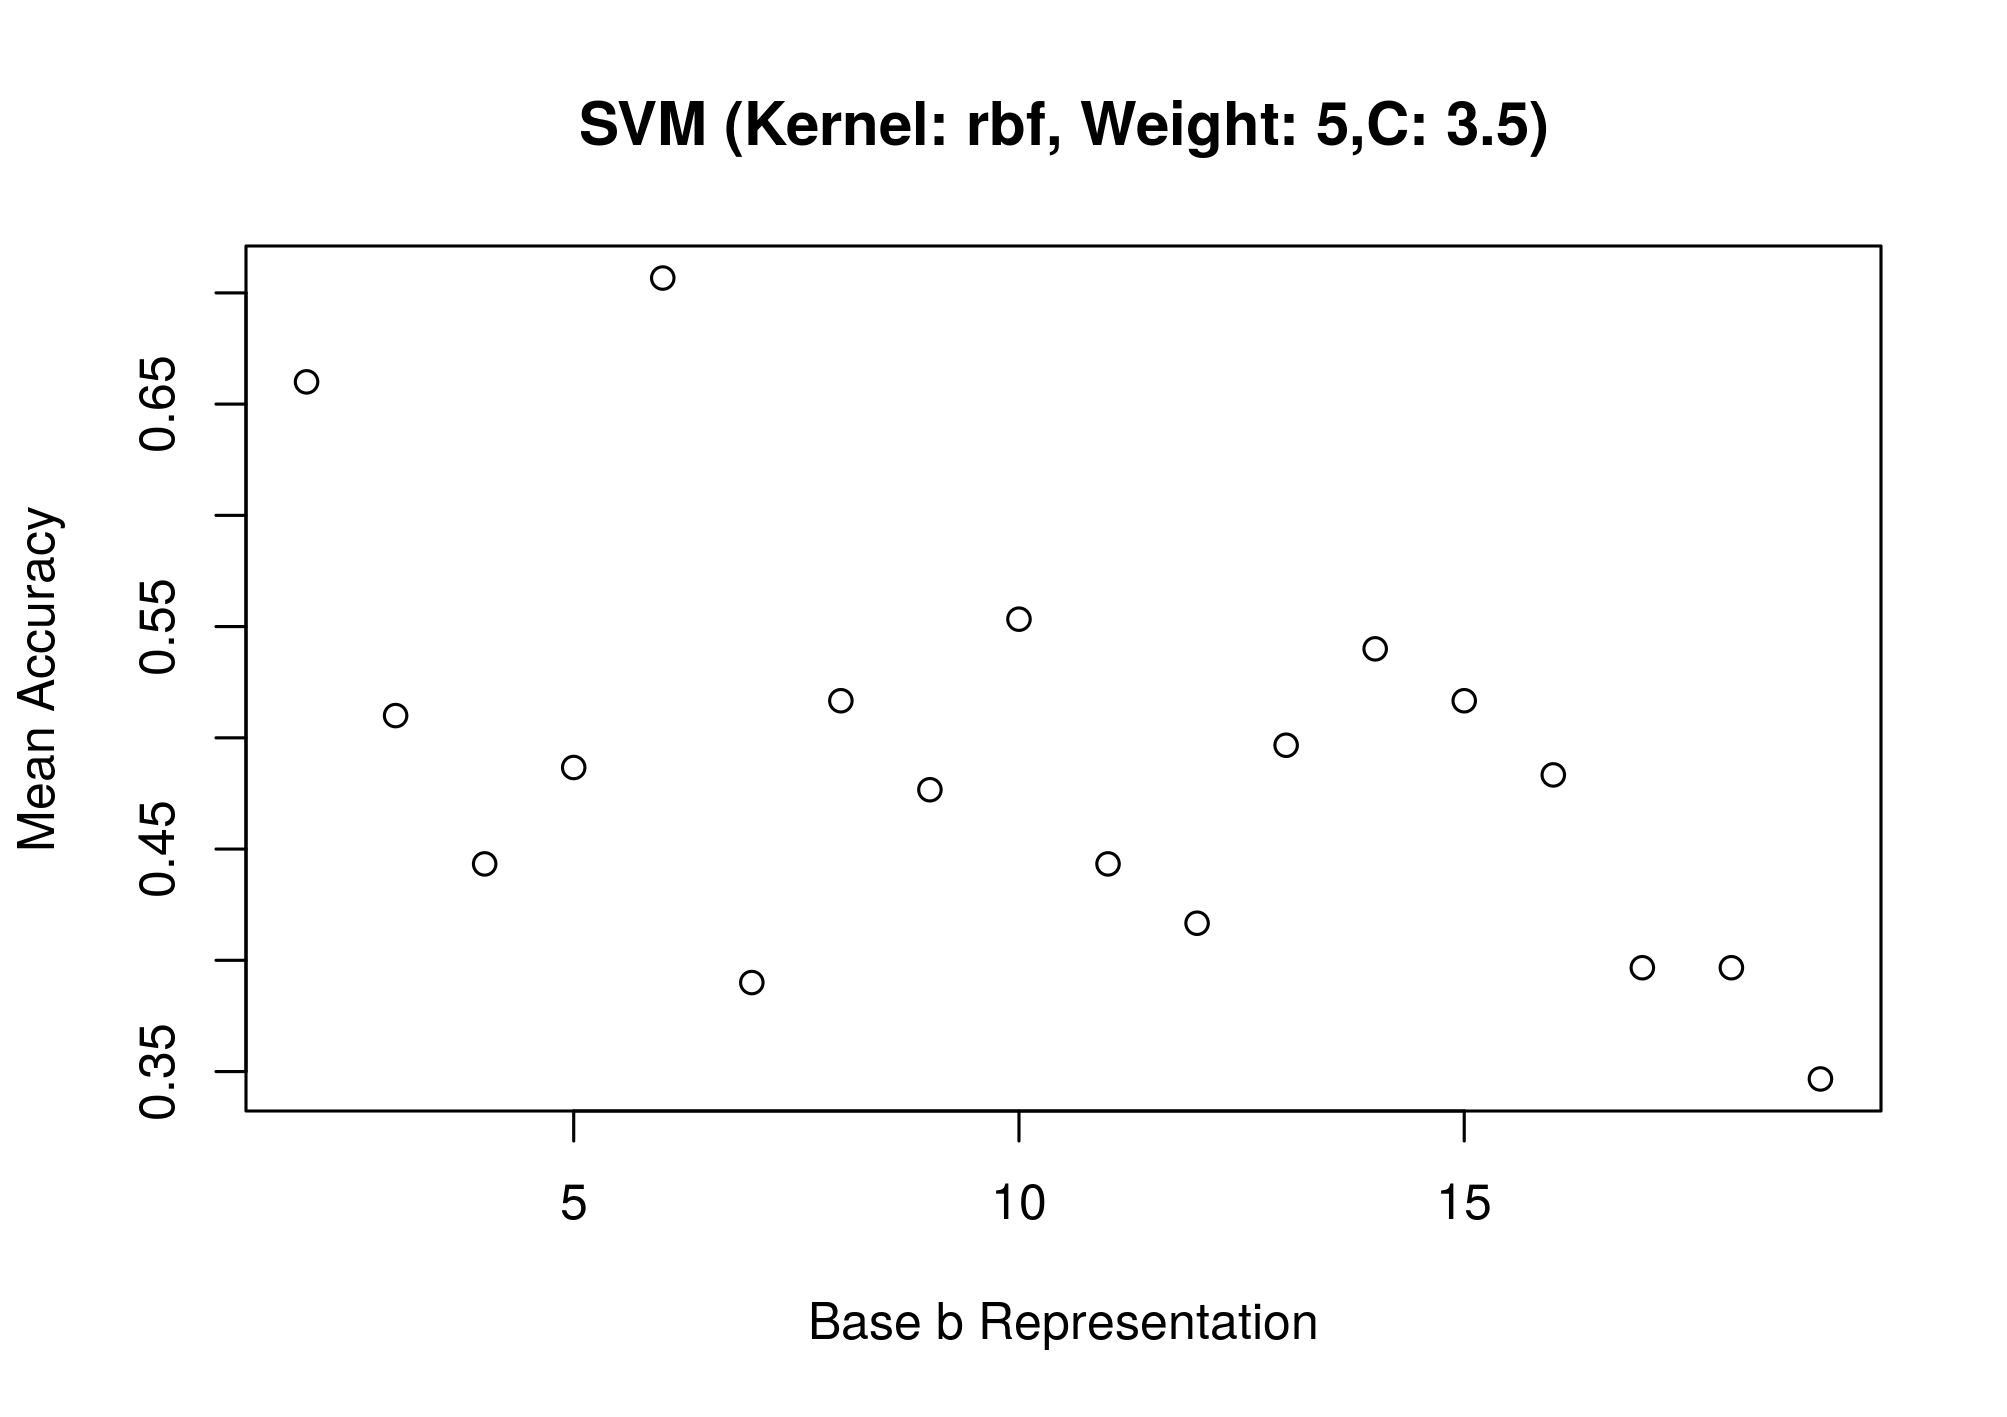
\includegraphics[width=\textwidth]{base_demo}
	\end{center}		
\end{frame}

\begin{frame}
	\frametitle{Best Models}
	
	\begin{table}[]
		\centering
		%\caption{My caption}
		%\label{my-label}
		\begin{tabular}{|c|c|c|c|}
			\hline
			\textbf{Base} & \textbf{C} & \textbf{Weight} & \textbf{Accuracy} \\ \hline
			6 & 3.2 & 2 & 0.86 \\ \hline
			6 & 3.7 & 2 & 0.86 \\ \hline
			6 & 3.8 & 2 & 0.86 \\ \hline
			6 & 3.9 & 2 & 0.86 \\ \hline
			6 & 4.0 & 2 & 0.86 \\ \hline
			6 & 4.1 & 2 & 0.86 \\ \hline
			6 & 4.7 & 2 & 0.86 \\ \hline
			6 & 4.8 & 2 & 0.86 \\ \hline
			6 & 4.9 & 2 & 0.86 \\ \hline
		\end{tabular}
	\end{table}
\end{frame}

\section{Conclusion}

\begin{frame}
	\frametitle{Conclusion}
	\begin{center}
		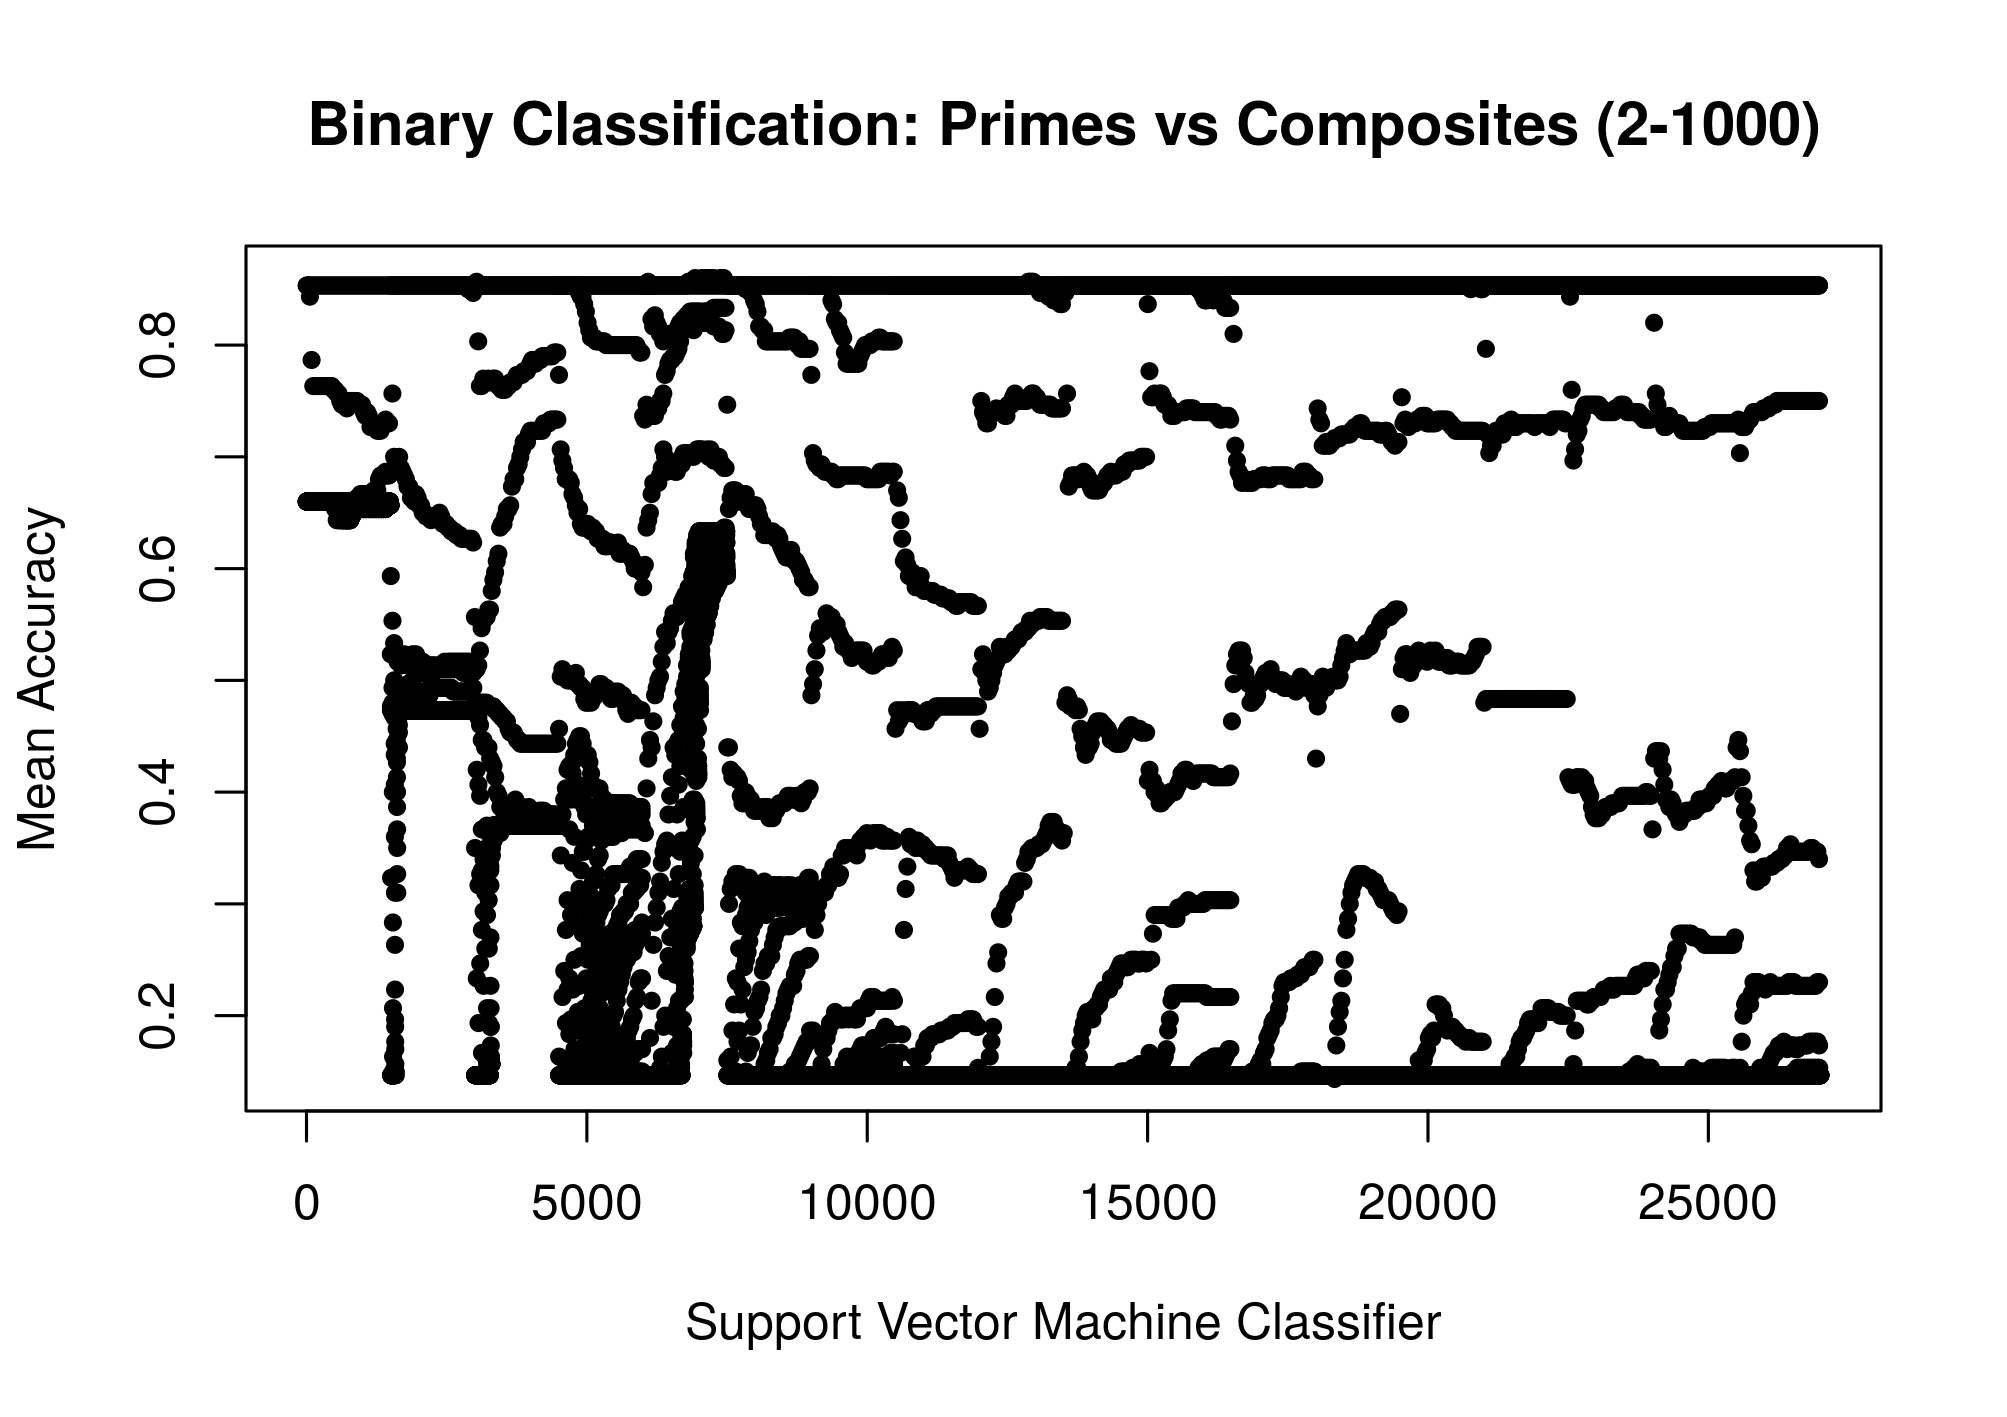
\includegraphics[width=\textwidth]{complete}
	\end{center}			
\end{frame}

\begin{frame}
	\frametitle{Sly Models}
	
	\begin{itemize}
		\item 168 primes between 2 and 1000 (inclusive)
		
		\begin{seqsplit}
			\tiny
			\{2, 3, 5, 7, 11, 13, 17, 19, 23, 29, 31, 37, 41, 43, 47, 53, 59, 61, 67, 71, 73, 79, 83, 89, 97, 101, 103, 107, 109, 113, 127, 131, 137, 139, 149, 151, 157, 163, 167, 173, 179, 181, 191, 193, 197, 199, 211, 223, 227, 229, 233, 239, 241, 251, 257, 263, 269, 271, 277, 281, 283, 293, 307, 311, 313, 317, 331, 337, 347, 349, 353, 359, 367, 373, 379, 383, 389, 397, 401, 409, 419, 421, 431, 433, 439, 443, 449, 457, 461, 463, 467, 479, 487, 491, 499, 503, 509, 521, 523, 541, 547, 557, 563, 569, 571, 577, 587, 593, 599, 601, 607, 613, 617, 619, 631, 641, 643, 647, 653, 659, 661, 673, 677, 683, 691, 701, 709, 719, 727, 733, 739, 743, 751, 757, 761, 769, 773, 787, 797, 809, 811, 821, 823, 827, 829, 839, 853, 857, 859, 863, 877, 881, 883, 887, 907, 911, 919, 929, 937, 941, 947, 953, 967, 971, 977, 983, 991, 997\}
			\end{seqsplit}
			
		\item 16.8\% prime and 83.2\% composite 
		
	\end{itemize}

\end{frame}

\begin{frame}
	\frametitle{
		Finding the Right $K$}
	\begin{center}
		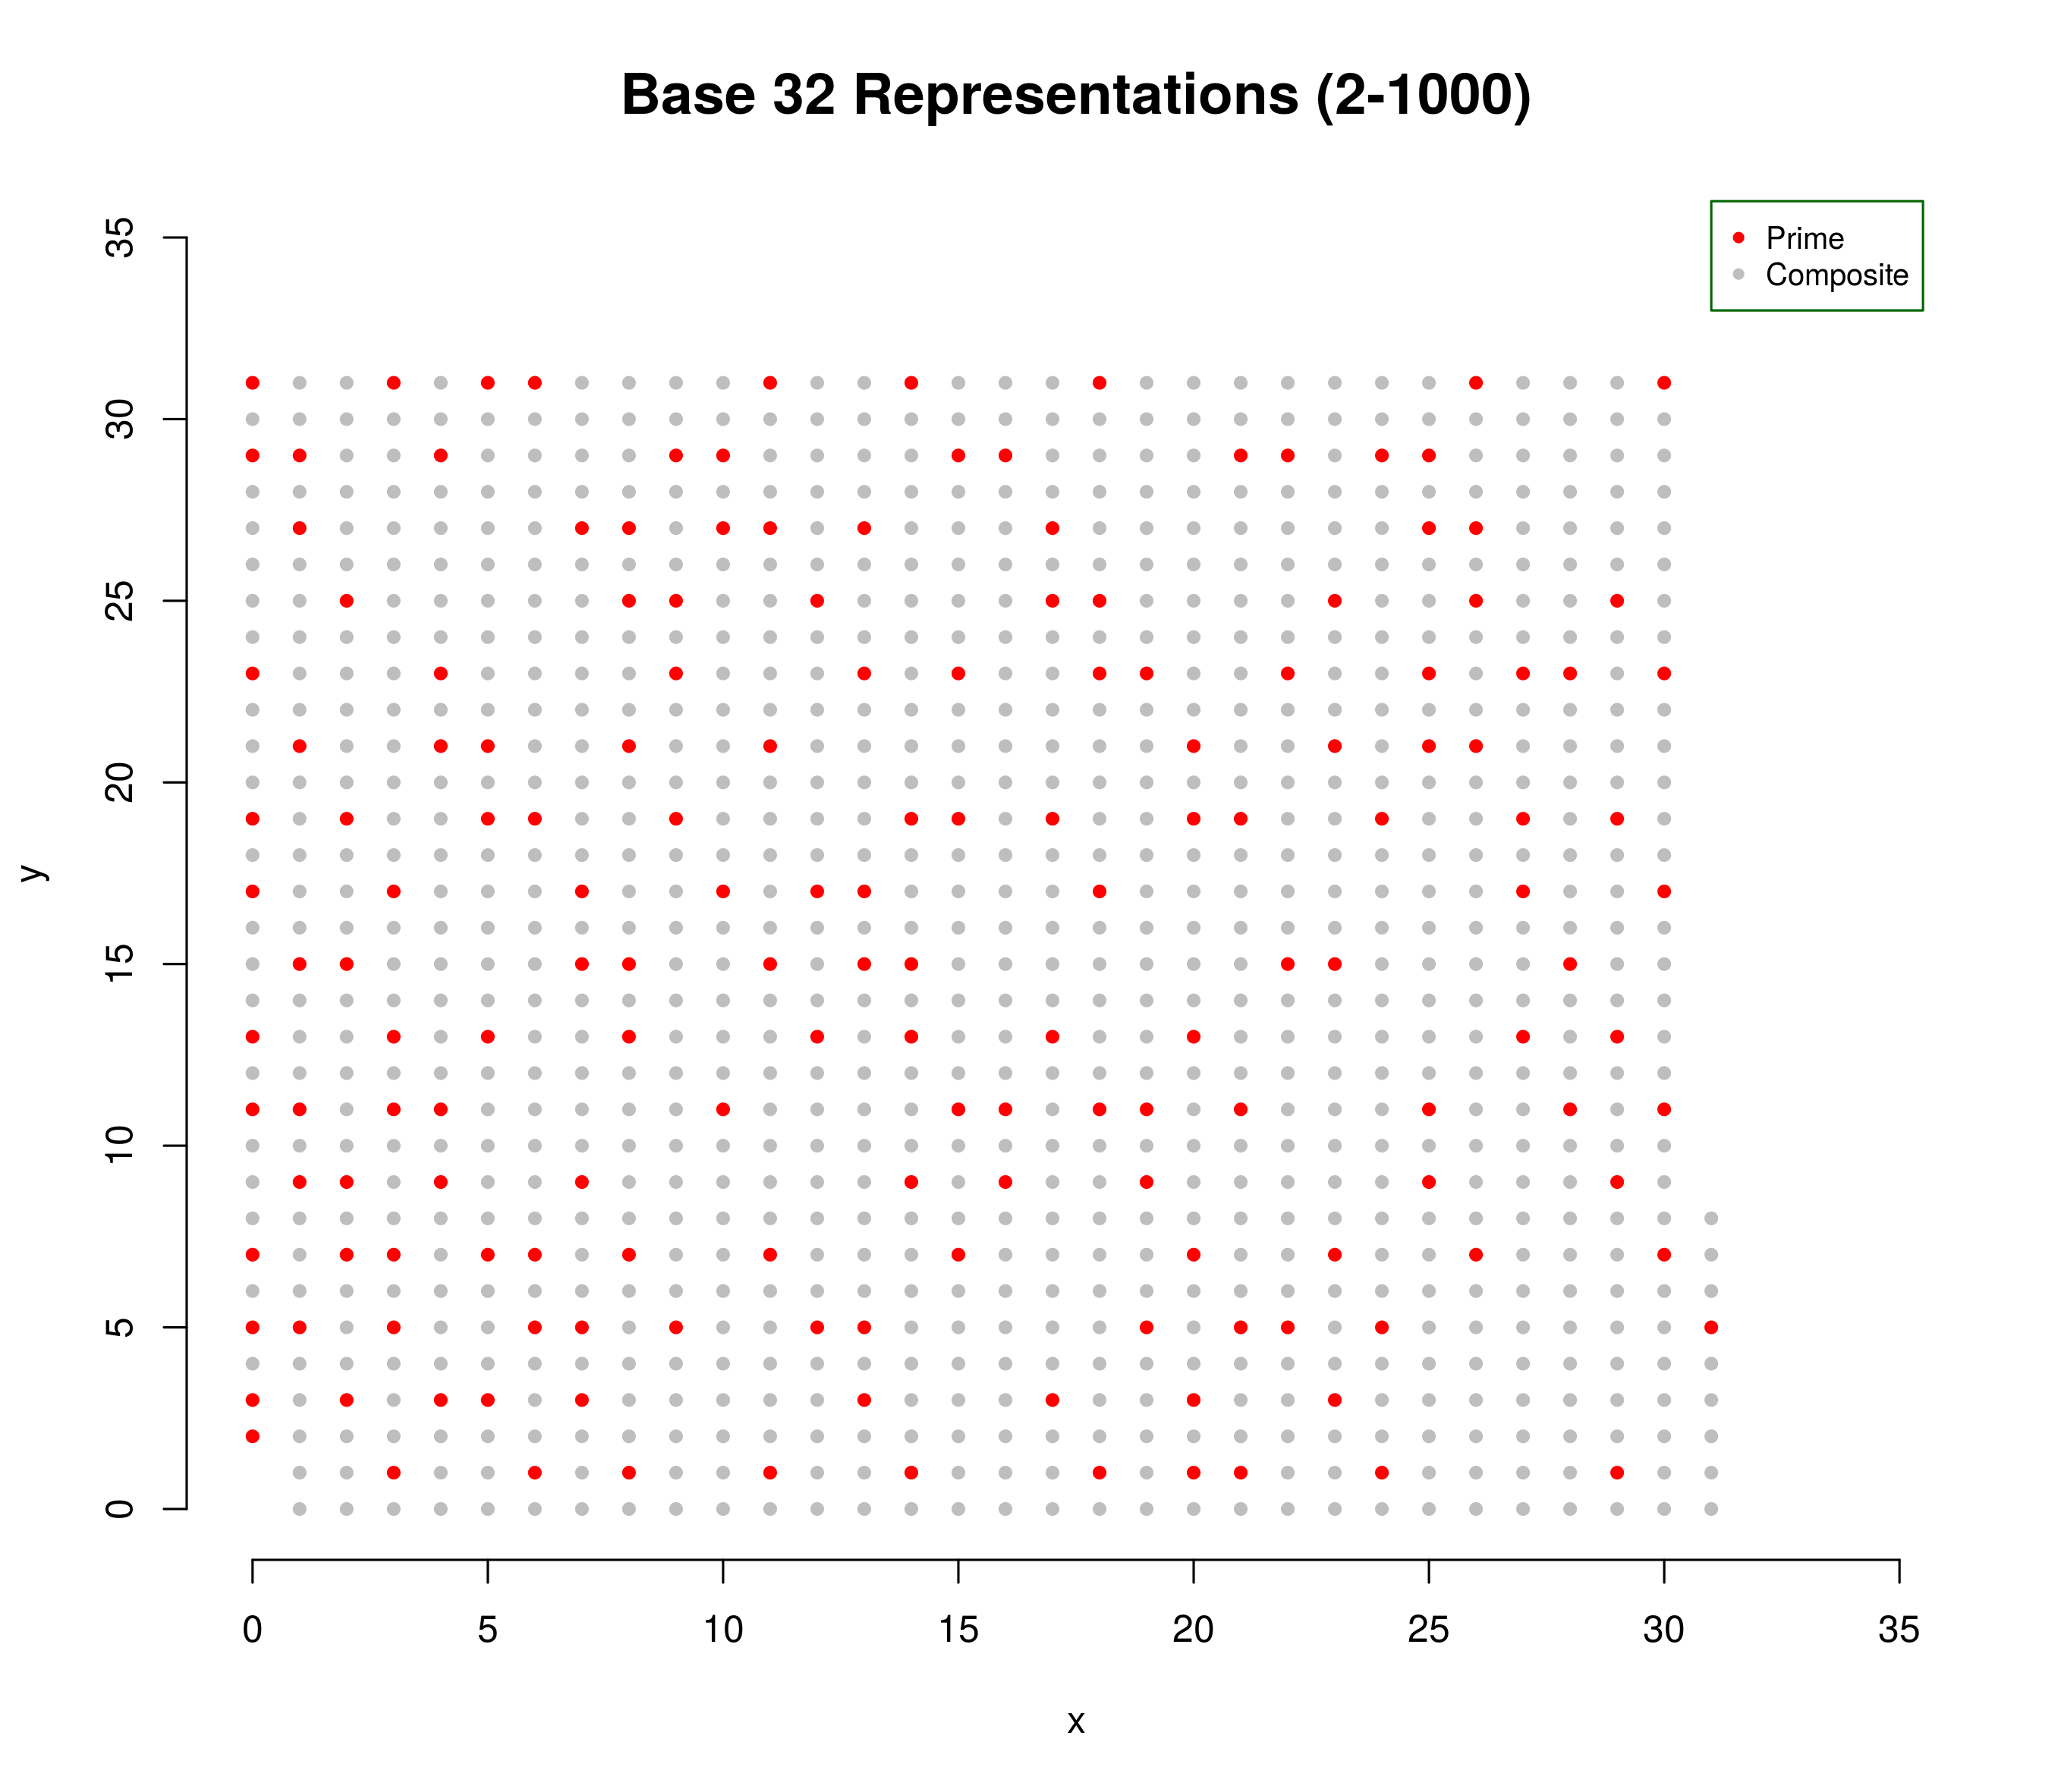
\includegraphics[height=0.88\textheight]{base_32}
	\end{center}			
\end{frame}


\begin{frame}
	\frametitle{References}
	\bibliographystyle{amsalpha}
	\bibliography{../report/refs.bib}	
\end{frame}

\begin{frame}
	\frametitle{Acknowledgements}
	\begin{itemize}
		\item My wife, Nora.
		\item Professor Tom Edgar
		\item Professor Yajun An
	\end{itemize}
\end{frame}

\begin{frame}
	\begin{lemma}\label{lemma:1_and_p-1_own_inverses}
		Let $p$ be prime. If $\bar{a} \in \Z_p$ is its own multiplicative inverse, then $\bar{a} = \bar{1}$ or $\bar{a} = \overline{p-1}$.
	\end{lemma}
	
	\begin{proof}
		Let $p \in \Z$ be prime, and let $\bar{a} \in \Z_p$ be its own multiplicative inverse.
		Then $\bar{a} \cdot \bar{a} = \bar{a}^2 = \bar{1}$; that is, $\bar{a}^2 - \bar{1} = (\bar{a} + \bar{1})(\bar{a} - \bar{1}) = \bar{0}$. 
		By the zero product property, since $\bar{a} + \bar{1} \in \Z_p$ and $\bar{a} - \bar{1} \in \Z_p$ and $(\bar{a} + \bar{1})(\bar{a} - \bar{1}) = \bar{0}$, then either $(\bar{a} + \bar{1}) = \bar{0}$ or $(\bar{a} - \bar{1}) = \bar{0}$. 
		We will consider both cases.
		
		\textbf{Case 1}. If $(\bar{a} + \bar{1}) = \bar{0}$, then $\bar{a} = -\bar{1} = \overline{p-1}$.
		
		\textbf{Case 2}. If $(\bar{a} - \bar{1}) = \bar{0}$, then $\bar{a} = \bar{1}$.
		
		\noindent Therefore, $\bar{a} = \bar{1}$ or $\bar{a} = \overline{p-1}$.
	\end{proof}
	

\end{frame}


\end{document}
